\begin{enumerate}[label=\thesection.\arabic*, ref=\thesection.\theenumi]
\item Find
	\begin{enumerate}
	\begin{multicols}{3}
	\item $2.7\times 4$
	\item $1.8\times 1.2$
	\item $2.3\times 4.35$
	\end{multicols}
	\end{enumerate}
and arrange the products in descending order.
\item Find the average of $4.2, 3.8$ and $7.6$.
\item Ashish studies for 4 hours, 5 hours and and 3 hours respectively on three consecutive days.  How many hours does he study daily on an average?
\item A batsman scored the following number of runs in 6 innings.  
	$$36, 35, 50, 46, 60, 55$$
	Calculate the mean runs scored by him in an inning.
\item The ages in years of 10 teachers of a school are
	$$32, 41, 28, 54, 35, 26, 23, 33, 38, 40$$
	\begin{enumerate}
		\item What is the age of the oldest teacher and that of the youngest teacher?
		\item What is the range of the ages of the teachers?
		\item What is the mean age of these teachers?
	\end{enumerate}
\item Organize the following marks in a class assessment, in tabular form with columns as marks and frequency.
	\begin{enumerate}
		\item Which number is the highest?
		\item Which number is the lowest?
		\item What is the range of the data?
		\item Find the arithmetic mean.
	\end{enumerate}
\item A cricketer scores the following runs in eight innings.
	$$58, 76, 40, 35, 46, 45, 0, 100$$
	Find the mean score.
\item Generate the following table using a C program
	\begin{figure}[H]
  \centering
  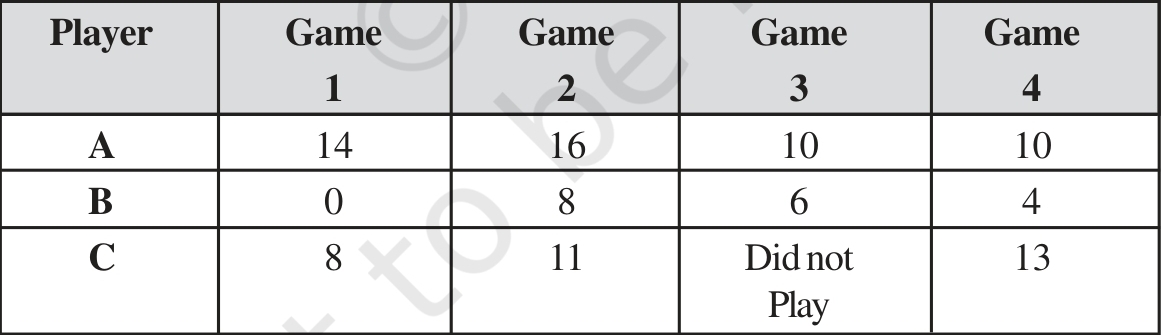
\includegraphics[width=\columnwidth]{figs/data.jpg}
  \caption{}
  \label{fig:data}
\end{figure}
and answer the following questions.
\begin{enumerate}
	\item Find the mean to determine $A's$ average number of points scored per game.
	\item Who is the best performer?
\end{enumerate}
\item The marks out of 100 obtained by a group of students in a science test are 85, 76, 90, 85, 39, 48, 56, 95, 81 and 75.  Find the 
	\begin{enumerate}
		\item Highest and lowest marks obtained by the students.
		\item Range of marks obtained.
		\item  Mean marks obtained by the group.
	\end{enumerate}
\item The enrolment in a school during six consecutive years was as follows  
	$$1555, 1670, 1750, 2013, 2540, 2820$$
	Find the mean enrolment of the school for this period.
\item The rainfall (in mm) in a city on 7 days a week was recorded as in 
  \tabref{fig:data2}.  Generate this table using a C program.
	\begin{figure}[H]
  \centering
  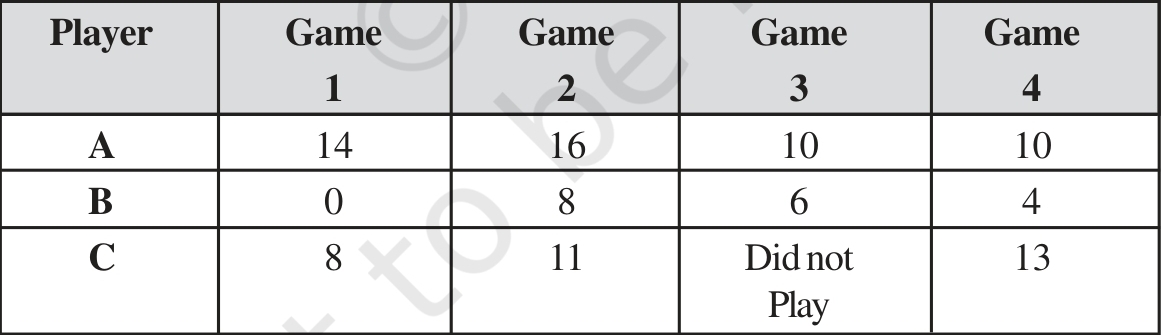
\includegraphics[width=\columnwidth]{figs/data.jpg}
  \caption{}
  \label{fig:data2}
\end{figure}
\item Find the range of the rainfall in the given data.
\item Find the mean rainfall for the week.
\item On how many days was the rainfall less than the mean rainfall 
\item The height of 10 girls was measured in cm and result was as follows
	$$135, 150, 139, 128, 151, 132, 146, 149, 143, 141.$$
	\begin{enumerate}
		\item What is the height of the tallest girl?
		\item What is the height of the shortest girl?
		\item What is the range of the data?
		\item What is the mean height of the girls?
		\item How many girls have heights more than the mean height?
	\end{enumerate}
\item To find out the weekly demand for different sizes of shirt, a shopkeeper kept records of sales of sizes as shown in 
  \eqref{fig:mode}.  This is the record for a week.  Find the mode of the data.
	\begin{figure}[H]
  \centering
  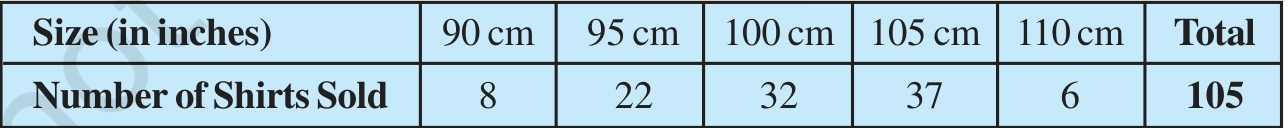
\includegraphics[width=\columnwidth]{figs/mode.jpg}
  \caption{}
  \label{fig:mode}
\end{figure}
\item Find the mode of the given set of numbers
	$$1,1,1,2,2,2,2,3,4,4$$.
\item Following are the margins of victory in the football matches of a league.  Find the mode of this data.
	\begin{gather*}
	1,3,2,5,1,4,6,2,5,2,2,2,4,1,2,3,1,1,2,3,2,6,4,3,2,
	\\
	1,1,4,2,1,5,3,3,2,3,2,42,1,2.
	\end{gather*}
\end{enumerate}
Find the mode of
\begin{enumerate}[label=\thesection.\arabic*, ref=\thesection.\theenumi,resume*]
\item 	
		\begin{gather*}
		2,6,5,3,0,4,3,2,4,5,2,4
	\end{gather*}
\item 
		\begin{gather*}
		2,4,16,12,14,14,16,14,10,14,18,14
	\end{gather*}
	\item 
		\begin{gather*}
		2,2,2,3,3,4,5,5,5,6,6,8
	\end{gather*}
	\item 
		\begin{gather*}
		12, 14, 12, 16, 15, 13, 14, 18, 19, 12, 14, 15, 16, 15, 16, 16,
	\\
		15, 17, 13, 16, 16, 15, 15, 13, 15, 17, 15, 14, 15, 13, 15, 14
		\end{gather*}
	\item Heights (in cm) of 25 children given below
		\begin{gather*}
		168, 165, 163, 160, 163, 161, 162, 164, 163, 162,
164, 163,	160, 
		\\
	 163, 160, 165, 163, 162, 163, 164, 163, 160, 165, 163, 162 
	\end{gather*}
		What is the mode of their heights? What do we understand by mode here?
\end{enumerate}
\begin{enumerate}[label=\thesection.\arabic*, ref=\thesection.\theenumi,resume*]
	\item 
Find the median of
		the group of 17 students with the following heights (in cm)
\begin{gather*}
106, 110, 123, 125, 117, 120, 112, 115, 
\\
110, 120, 115, 102, 115, 115, 109, 115, 101
\end{gather*}
\item Your friend found the median and the mode of a given data. Describe and correct your friends error if any
\begin{gather*}
	35, 32, 35, 42, 38, 32, 34 
\end{gather*}
Median = 42, Mode = 32.
\item Find the median of the data: 24, 36, 46, 17, 18, 25, 35.
\item The scores in mathematics test (out of 25) of 15 students is as follows
	\begin{gather*}
	19, 25, 23, 20, 9, 20, 15, 10, 5, 16, 25, 20, 24, 12, 20 
\end{gather*}
Find the mode and median of this data. Are they same?
\item The runs scored in a cricket match by 11 players is as follows 
	\begin{gather*}
	6, 15, 120, 50, 100, 80, 10, 15, 8, 10, 15
\end{gather*}
Find the mean, mode and median of this data. Are the three same?
\item The weights (in kg.) of 15 students of a class are
	\begin{gather*}
	38, 42, 35, 37, 45, 50, 32, 43, 43, 40, 36, 38, 43, 38, 47
\end{gather*}
\begin{enumerate}
	\item  Find the mode and median of this data. 
	\item Is there more than one mode?
\end{enumerate}
\item Find the mode and median of the data
	\begin{gather*}
	13, 16, 12, 14, 19, 12, 14, 13, 14
\end{gather*}
\item
	The data 
	\begin{gather*}
	6, 4, 3, 8, 9, 12, 13, 9 
\end{gather*}
has mean 9.  True or False?
\item Two hundred students of 6th and 7th classes were asked to name their favourite colour so as to decide upon what should be the colour of their school building. The results are shown in the following table
  in \figref{fig:bar}.
	 Represent the given data on a bar graph
	\begin{figure}[H]
  \centering
  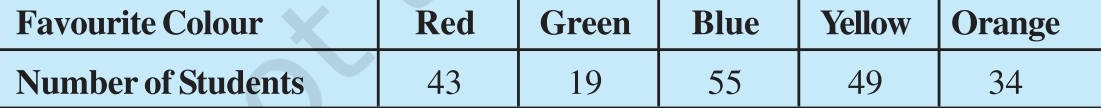
\includegraphics[width=\columnwidth]{figs/bar.jpg}
  \caption{}
  \label{fig:bar}
\end{figure}
Answer the following questions with the help of the bar graph
	\begin{enumerate}
	\item Which is the most preferred colour and which is the least preferred? 
	\item How many colours are there in all? What are they?
	\end{enumerate}
\item Following data 
  in \figref{fig:bar1}
	gives total marks (out of 600) obtained by six children of a particular class. Represent the data on a bar graph.
	\begin{figure}[H]
  \centering
  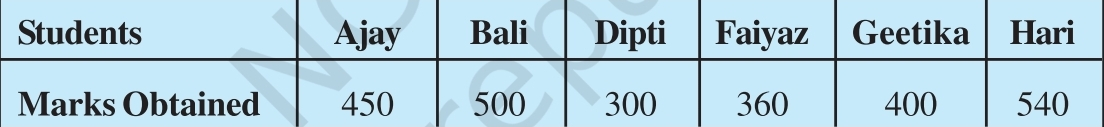
\includegraphics[width=\columnwidth]{figs/bar1.jpg}
  \caption{}
  \label{fig:bar1}
\end{figure}
\item Consider the following two collections of data 
in
\figref{fig:bar2}
	giving the average daily hours of sunshine in two cities Aberdeen and Margate for all the twelve months of the year. These cities are near the south pole and hence have only a few hours of sunshine each day.
	In a particular month, which city has more sunshine hours?  Explain through a double bar graph.
	\begin{figure}[H]
  \centering
  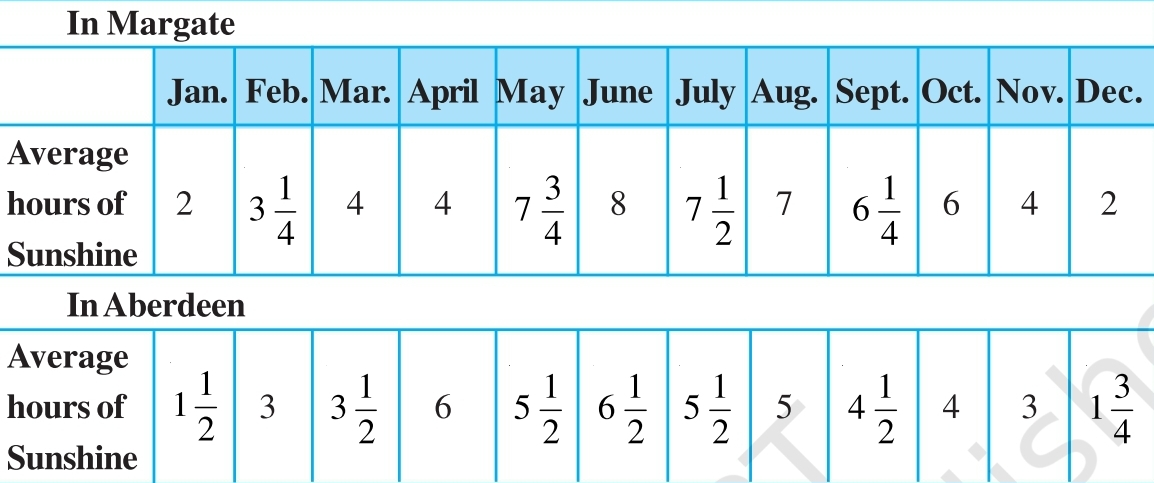
\includegraphics[width=\columnwidth]{figs/bar2.jpg}
  \caption{}
  \label{fig:bar2}
\end{figure}
\end{enumerate}
